\section{System Architecture}
\label{sec:system}


The overall system architecture is illustrated in Figure~\ref{fig:donnie-sys}. The student uses a computer (Figure~\ref{fig:donnie-sys}(a)) with wifi connectivity to remotely connect to either the physical robot (Figure~\ref{fig:donnie-sys}(c)) or the virtual simulation environment (Figure~\ref{fig:donnie-sys}(b)). Both physical and virtual robots are equivalent, except that the physical robot also uses vibration as an assistive aid. The student's computer has the proposed assistive IDE that includes textual interfaces, screen readers, magnification software. The student programs in Logo-based language which translates the commands/sensors to the Player robotic framework. Player sends the commands to the robot and receives robot sensors inputs to display it at the console or in log files. The next sections details the robot's hardware (Section~\ref{sec:hardware}) and software (Section~\ref{sec:software}) designs.

\begin{figure}[h!]
  \centering
    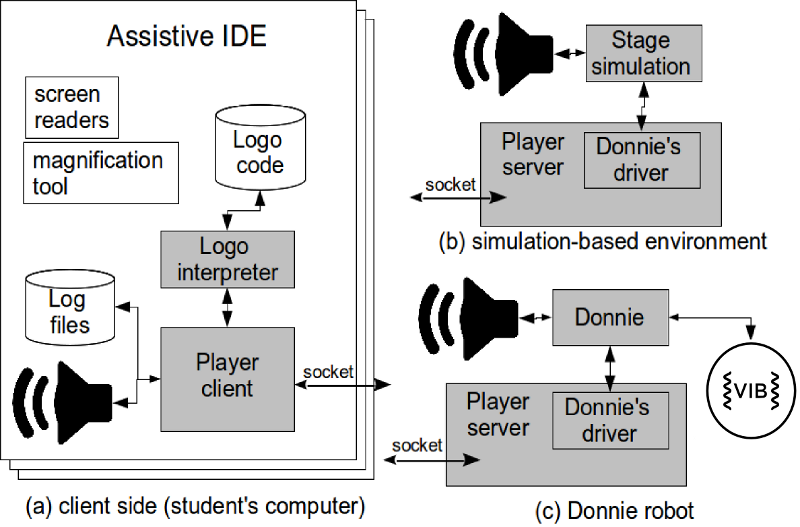
\includegraphics[width=0.95\linewidth]{figs/assistive-env.png}
  \caption{Donnie's system architecture.}
  \label{fig:donnie-sys}
\end{figure}


%%%%%%%%%%%%%%%%%%%%%%%%%%%%%%%%%%%%%%%%%%%%%%%%%%%%%%%

\subsection{Hardware Architecture}
\label{sec:hardware}

The hardware architecture consists of an open mechanical model \footnote{\url{https://github.com/lsa-pucrs/donnie-assistive-robot-3d}}, which can be built with a 3D printer, and an open electronic system \footnote{\url{https://github.com/lsa-pucrs/donnie-assistive-robot-hw}} based on Raspberry Pi and Arduino. Both boards were chosen due to their availability in the market, low cost, and the size of the developer community, which eases the addition of new capabilities in the future. Moreover, both boards are used in several educational projects, thus, the schools might already have some of these boards.

\subsubsection{The Mechanical Model}
\label{sec:mech}

Figure~\ref{fig:donnie-mech} illustrates Donnie's mechanical model and an example of 3D printed robot. Its main mechanical features include:

\begin{itemize}
\item It is a differential robot with two parallel wheels;
\item It has one bumper in the front and another in the rear;
\item It has a head that can turn to left and right-hand sides to scan the surroundings;
\item It has seven sonar sensors for obstacle avoidance;
\item It has a modular design, divided into stacks, such that an additional stack can be added on demand.
\end{itemize}



\begin{figure}[h!]
    \centering
    \begin{subfigure}[b]{0.8\linewidth}
        \centering
        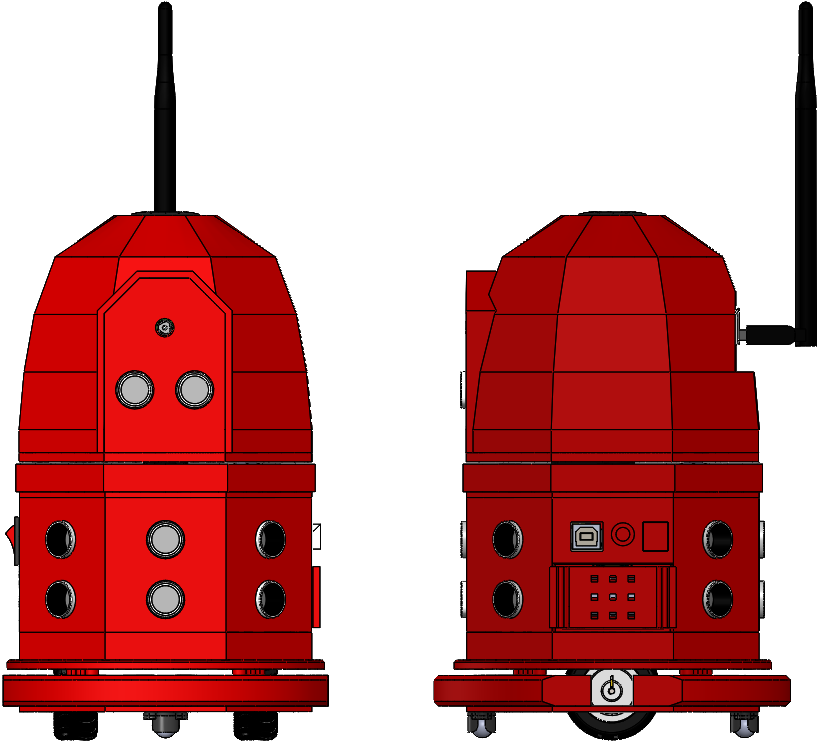
\includegraphics[width=\linewidth]{figs/donnie-3d_model.png}
        \caption{3D model.}
    \end{subfigure}
    ~
    \begin{subfigure}[b]{0.8\linewidth}
        \centering
        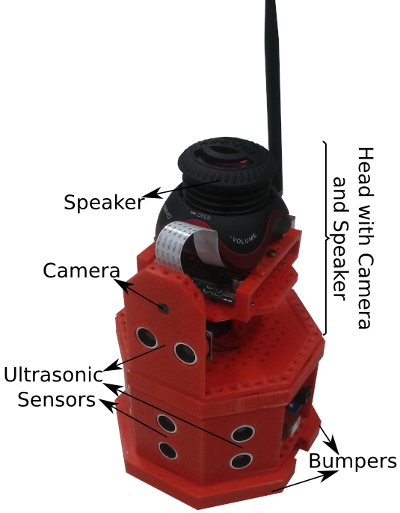
\includegraphics[width=\linewidth]{figs/donnie-printed.png}
        \caption{3D printed robot.}
    \end{subfigure}
    \caption{Donnie's mechanical model.}
    \label{fig:donnie-mech}
\end{figure}


%\begin{figure}[h!]
%  \centering
%    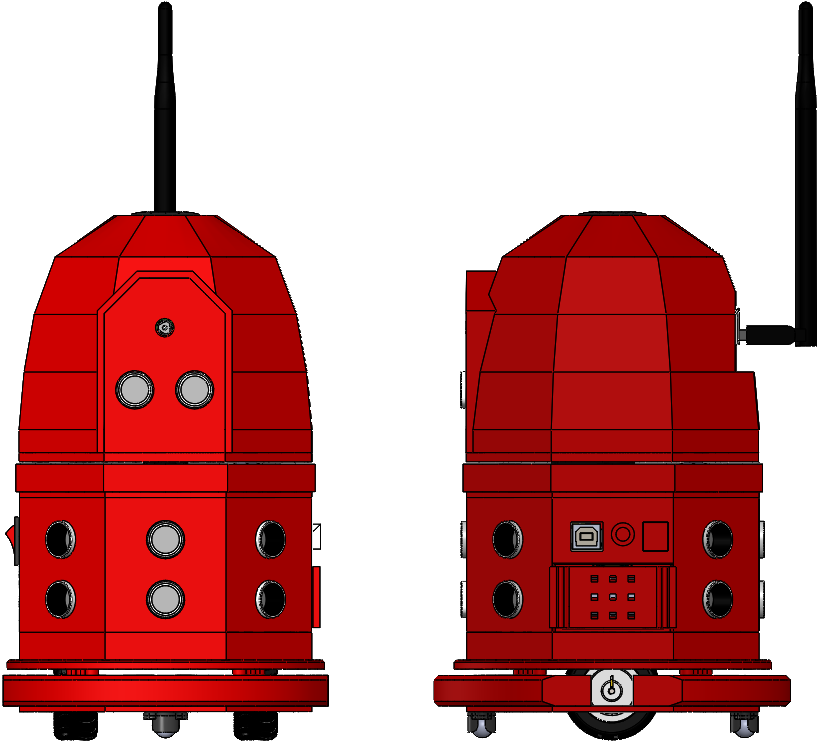
\includegraphics[width=0.5\textwidth]{figs/donnie-3d_model.png}
%  \caption{Donnie`s 3D Model.}
%  \label{fig:donnie-3d_model}
%\end{figure}

Currently Donnie has three stacks. The lower stack (the feet) is for the wheels, the motors, the motor encoders, and the bumpers. The second stack (the body) has the battery, six ultrasonic sensors, and the Arduino board. The third one (the head) has one ultrasonic sensor, the camera, the speaker, and the Raspberry Pi board. Additional stacks can be mounted in between the existing stacks to add new functionality.

%%%%%%%%%%%%

\subsubsection{The Electronic System}
\label{sec:elet}

Figure~\ref{fig:donnie-elet} illustrates Donnie's electronic systems which is divided in two main parts: Arduino and Raspberry Pi (RPi). While the RPi board does the interface to the robot`s peripheral which are similar to a computer peripheral (i.e. camera, speaker, wifi), the Arduino board does the interface to the IO resources exclusive for robots (range sensors, motors, encoders, etc). 

\begin{figure}[h!]
  \centering
    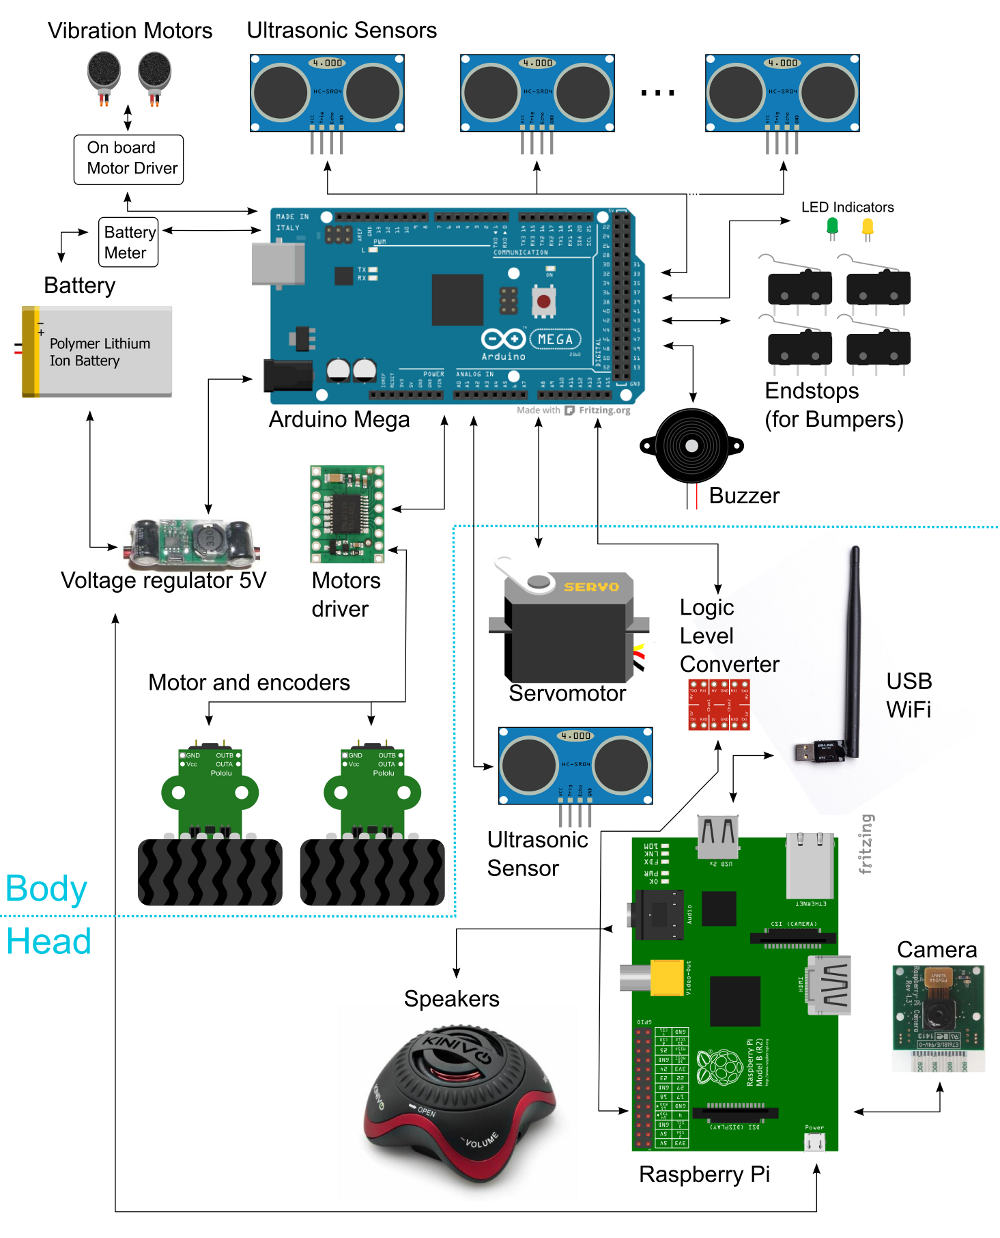
\includegraphics[width=0.95\linewidth]{figs/donnie-elet.png}
  \caption{Donnie's Electronic System: (a) Arduino and (b) Raspberry Pi.}
  \label{fig:donnie-elet}
\end{figure}

The design decision to use two boards (Arduino and RPi) instead of only one of them is discussed as follows. For instance, it would be possible to implement all peripherals using only the RPi board. However, this would lead to a reduced number of interfaces for future expansions and add-ons. By using an Arduino Mega, there are enough interfaces for several new features such as, for example, a gripper, line following sensors, among other possible extensions. Alternatively, there are few expansion boards for RPi for robotics \footnote{\url{https://www.adafruit.com/products/1940}} \footnote{\url{https://www.piborg.org/picoborgrev}} that could also be used instead of the Arduino Mega. The advantage of Arduino is its availability, large user community, and it can be removed from the robot and used alone to teach programming \cite{ardu-book1,ardu-book2}. This way, Arduino is a more versatile option than the RPi expansion boards. On the other hand, there are also several robot proposal using only Arduino boards. The main drawback of these approaches is that they provide limited computing capability, limiting the learning experience. The robot would become obsolete as soon as the student acquire the basic programming skill enabled by an Arduino board. This way, by combining both Arduino and RPi boards the robot become modular, expandable, and also with good computing capabilities to enable advanced programming and robotics learning. Both boards are also well documented, with several books about robotics such as \cite{rpi-book1,rpi-book2,rpi-book3} and \cite{ardu-book1, ardu-book2}.

As illustrated in Figure~\ref{fig:donnie-elet}, the Arduino board communicates with the Raspberry Pi board using the serial interface via a level shifter. The firmware running on the Arduino is explained in Section~\ref{sec:firm}. As illustrated in Figure~\ref{fig:donnie-elet}, the Arduino board is located at the robot's body and it controls:

\begin{enumerate}
\item The DC driver and two motors to move the robot;
\item The motor encoders that evaluate the distance travelled by each motor;
\item The buzzer and the vibrating motor used for assistive interface in case of robot collision, obstacle detection, low battery alert;
\item The LEDs provide similar feedback as mentioned before for students with normal vision;
\item The two tactile bump sensors, each one using two switches, used to detect collisions; 
\item The battery sensor used to indicate low battery;
\item The servo motor to implement the head movement for scanning the surroundings with head`s sonar and the camera (RaspiCam v1 with OmniVision OV5647 Color CMOS sensor);
\item Seven sonar sensors (including the one in the head) for navigation and obstacle avoidance;
\item The level shifter to adapt the serial voltage between the Arduino and the RPi boards.
\end{enumerate}

The Raspberry Pi board runs a Linux operating system with Raspbian distribution. This board runs the Donnie's device driver (Section~\ref{sec:driver}) and it also controls the camera (and its image processing), the sound at the speaker, and the wifi connectivity. 


%\todo{Marques e Augusto: falar das placas desenvolvidas. Favor preencher estas informações}

Two additional boards were developed to connect the robot's electrical components. The first board is a 3.6 by 4.2 cm board, with two layers, used to connect the RPi board with the electronics in the head (ultrasonic sensor and servo motor) with the Arduino board. The second board is attached to the Arduino board. It has 6.3 by 10.6 cm and two layers. It contains six ultrasonic connectors, two vibration motor drivers, one battery voltage meter, four digital bumper inputs, two leds, one buzzer output, two encoder inputs, and a motor driver to control two DC motors. This board has a connector to communicate with the first board. Both boards are illustrated in Figure~\ref{fig:donnie-boards}.


\begin{figure}[h!]
    \centering
    \begin{subfigure}[b]{0.60\linewidth}
        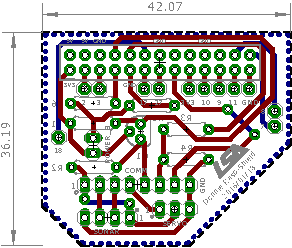
\includegraphics[width=\linewidth]{figs/rasp_shield_v1_eagle_brd.pdf}
        \caption{RPi board Layout.}
    \end{subfigure} %
    \begin{subfigure}[b]{0.85\linewidth}
        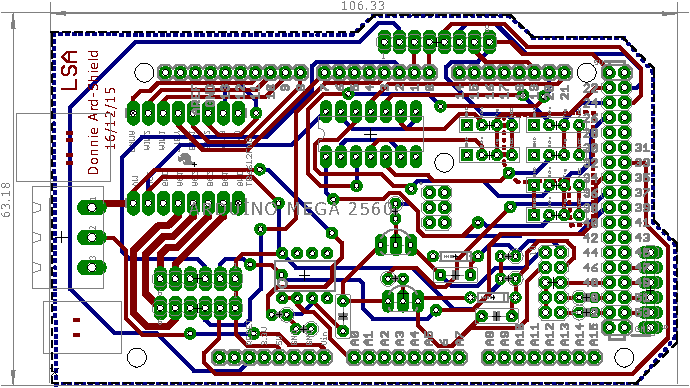
\includegraphics[width=\linewidth]{figs/arduino_shield_v1_eagle_brd.pdf}
        \caption{Arduino board Layout.}
    \end{subfigure}
%    \begin{subfigure}[b]{0.45\linewidth}
%        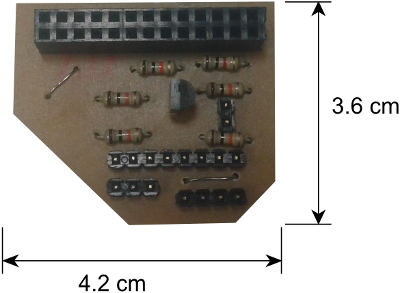
\includegraphics[width=\linewidth]{figs/rasp_board_v1.png}
%        \caption{Photo of the RPi board.}
%    \end{subfigure}
%    %\hspace{\fill} %
%    \hspace*{-0.6em} %
%    \begin{subfigure}[b]{0.45\linewidth}
%        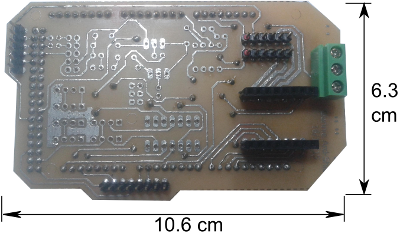
\includegraphics[width=\linewidth]{figs/arduino_board_v1.png}
%        \caption{Photo of the Arduino board.}
%    \end{subfigure}    
    \caption{Donnie's auxiliar boards.}
    \label{fig:donnie-boards}
\end{figure}



%%%%%%%%%%%%

\subsubsection{The Hardware Cost}
\label{sec:hw-cost}

The estimated cost to build a Donnie robot is US\$ 255 in electronics assuming none of the parts listed before are available. The amount of plastic required for 3D printing the robot is about 0.44 Kg. Assuming the plastic costs US\$48 per Kilo, the 3D printing cost is US\$ 21. 

The Table~\ref{tab:cost-table} shows the price of each component used to build Donnie, compared with the price of the equivalent parts of Lego's Mindstorms. The 'X' represents that the Lego does not have an equivalent official part and the '-' represents the item is not needed because it is included into the main part. For example, the Brick Mindstorm, that is build with an ARM9 micro processor, has an embedded speaker and Wi-Fi support, thus, it is not required to buy a separate piece. 
Few accessories were required to make Lego's Mindstorms more comparable with Donnie. Even though, Donnie still has advantages such as a better processor (able to run more complex codes and image processing), it has more sensors than Lego's robot, and it costs half the cost of an equivalent Lego's robot. 


\begin{table}[ht!]
\centering
\caption{The price table of Donnie's parts in comparison with Lego's Mindstorms equivalent parts.}
\label{tab:cost-table}
\begin{tabular}{|l|c|c|}
\hline
 & Donnie (U\$)    & Lego Mindstorms (U\$)  \\ \hline
motor driver             & 8.95    & -      \\ \hline
motor, encoder and wheel & 39.95   & 24.99  \\ \hline
micro controller         & 37.09   & 179.99 \\ \hline
servo                    & 19.95   & 19.99  \\ \hline
buzzer                   & 1.49    & X      \\ \hline
ultrasonic sensors       & 7*2.50  & 7*19.99\\ \hline
raspberry pi B           & 39.90   & X      \\ \hline
ubec                     & 5.98    & -      \\ \hline
camera                   & 29.95   & X      \\ \hline
usb wifi                 & 19.05   & -      \\ \hline
bumpers                  & 4*1.99  & 4*24.99\\ \hline
battery                  & 14.86   & 79.99  \\ \hline
speaker                  & 12.99   & -      \\ \hline
plastic                  & 21.00   & -      \\ \hline
\textbf{TOTAL (U\$)}     & \textbf{276.62} & \textbf{544.85}           \\ \hline
\end{tabular}
\end{table}

